\documentclass{beamer}
\usetheme{CambridgeUS}
\usecolortheme{dolphin}
%themes to test
%Theme to: AnnArbor Antibes Bergen Berkeley Berlin Boadilla boxes CambridgeUS Copenhagen Darmstadt default Dresden Frankfurt Goettingen Hannover Ilmenau JuanLesPins Luebeck Madrid Malmoe Marburg Montpellier PaloAlto Pittsburgh Rochester Singapore Szeged Warsaw
%Color to: albatross beaver beetle crane default dolphin dove fly lily orchid rose seagull seahorse sidebartab structure whale wolverine
%Font to: default professionalfonts serif structurebold structureitalicserif structuresmallcapsserif

\usepackage{graphicx} %allows picture file insertion into document
\usepackage{ulem} %allows strikethough (\sout)
\usepackage{amsmath}
\usepackage{comment}
\usepackage{multicol}

%sets numbered citation and uses bib.bib as bibliography file
\usepackage[natbib=true, style=numeric-comp, sorting=none]{biblatex}
\renewcommand*{\bibfont}{\tiny}
\addbibresource{lecture-cpr-by-race.bib}
\newcommand{\pro}{\textcolor{blue}}
\newcommand{\con}{\textcolor{red}}
\newcommand{\me}{Eric W. Robbins, MD}

\setbeamerfont{footnote}{size=\tiny} %sets size of footnote citation to \tiny

\title{Racial and Ethnic Differences in Bystander CPR \\ for Witnessed Cardiac Arrest}
\author{\me}
\date{Last updated: \today}
\begin{document}
	\begin{frame}
		\maketitle
	\end{frame}
	\begin{frame}
		\frametitle{Table of Contents}
			%\begin{multicols}{2}
				\tableofcontents
			%\end{multicols}
	\end{frame}
\section{Study Overview}
	\subsection{Study Questions}
		\begin{frame}
			\begin{figure}
				\centering
				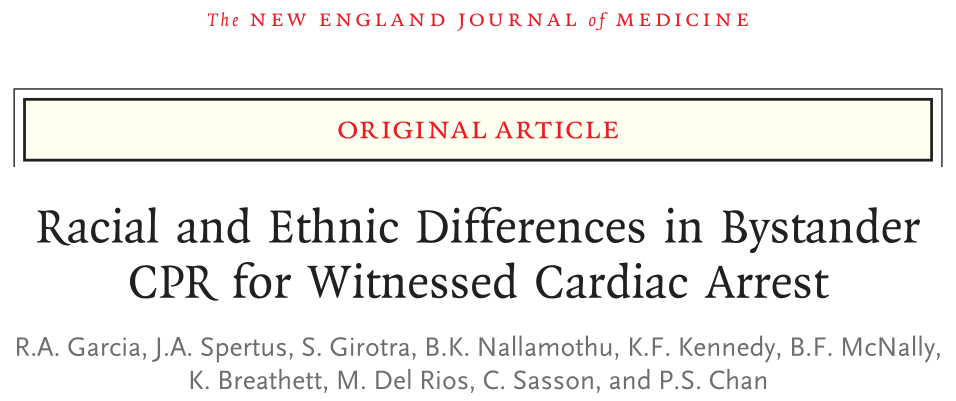
\includegraphics[width=1.0\linewidth]{img/headline}
				\label{fig:headline}
			\end{figure}
		\end{frame}
		\begin{frame}
			\frametitle{Study Questions}
				\begin{itemize}
					\item \textbf{Primary}
						\begin{itemize}
							\item Are there significant differences in the rates that Black and Hispanic patients receive bystander CPR for \textit{witnessed} cardiac arrests?
						\end{itemize}
					\item \textbf{Secondary}
					\begin{itemize}
						\item Do the above rates change according to neighborhood racial makeup, neighborhood income, or where the arrest occurs (at home versus in public)?
					\end{itemize}
					\item \textbf{Exploratory}
					\begin{itemize}
						\item Do Black and Hispanic patients have worse outcomes after adjusting for the above variables?
					\end{itemize}
				\end{itemize}
		\end{frame}
	\subsection{Historical Context}
		\begin{frame}
			\frametitle{Historical Context}
			\begin{itemize}
				\item ``Previous studies have shown that Black and Hispanic persons are less likely than White persons to receive bystander CPR after out-of-hospital cardiac arrest.''\cite{sasson_association_2012}
				\item Prior studies have shown lower incidence of CPR training in Black and Hispanic communities \cite{anderson_rates_2014}
				\item Hispanic bystanders are less likely to call 911 for due to distrust of law enforcement, perceived cost of ambulances, and fear of immigration status issues \cite{sasson_barriers_2015}
				\item Language barriers for 911 dispatchers delays start of CPR
					\begin{itemize}
						\item in one study, 116.5 second delay to start of CPR!\cite{nuno_disparities_2017}
					\end{itemize}
			\end{itemize}
		\end{frame}
	\subsection{What this Study Adds}
		\begin{frame}
		\frametitle{What this Study Adds}
			\begin{itemize}
				\item \textit{Witnessed} arrests only
				\item Differences between CPR responses:
					\begin{itemize}
						\item by neighborhood racial makeup
						\item by neighborhood economic makeup
						\item in public versus private spaces
					\end{itemize}
			\end{itemize}
		\end{frame}
	\subsection{Study Design}
		\begin{frame}
			\begin{itemize}
				\item Cardiac Arrest Registry to Enhance Survival (CARES) Database
					\begin{itemize}
						\item Established by CDC and Emory University
						\item Catchment of 167 million residents (51\% of US)
						\item Includes all non-traumatic out-of-hospital cardiac arrests for whom:
							\begin{enumerate}
								\item CPR was attempted
								\item identified by EMS agencies
							\end{enumerate}
					\end{itemize}
				\item Time period: January 1, 2013 -- December 31, 2019
				\item Data reporting:
					\begin{itemize}
						\item ``Neighborhoods'' were US census tracts
						\item Racial and income data from 2019 American Community Survey
						\item Racial data reported by patient, family member, or EMS personnel (only when person dies or no one else can provide information)
					\end{itemize}
				\item Outcome Definition:
					\begin{itemize}
						\item Initiation of bystander CPR by any layperson
							\begin{itemize}
								\item family member, medical provider, or other person who was NOT a 911 responder
							\end{itemize}
					\end{itemize}
			\end{itemize}
		\end{frame}
		\subsubsection*{Patient Selection}
			\begin{frame}
				\frametitle{Patient Selection from CARES Database}
				\begin{figure}
					\centering
					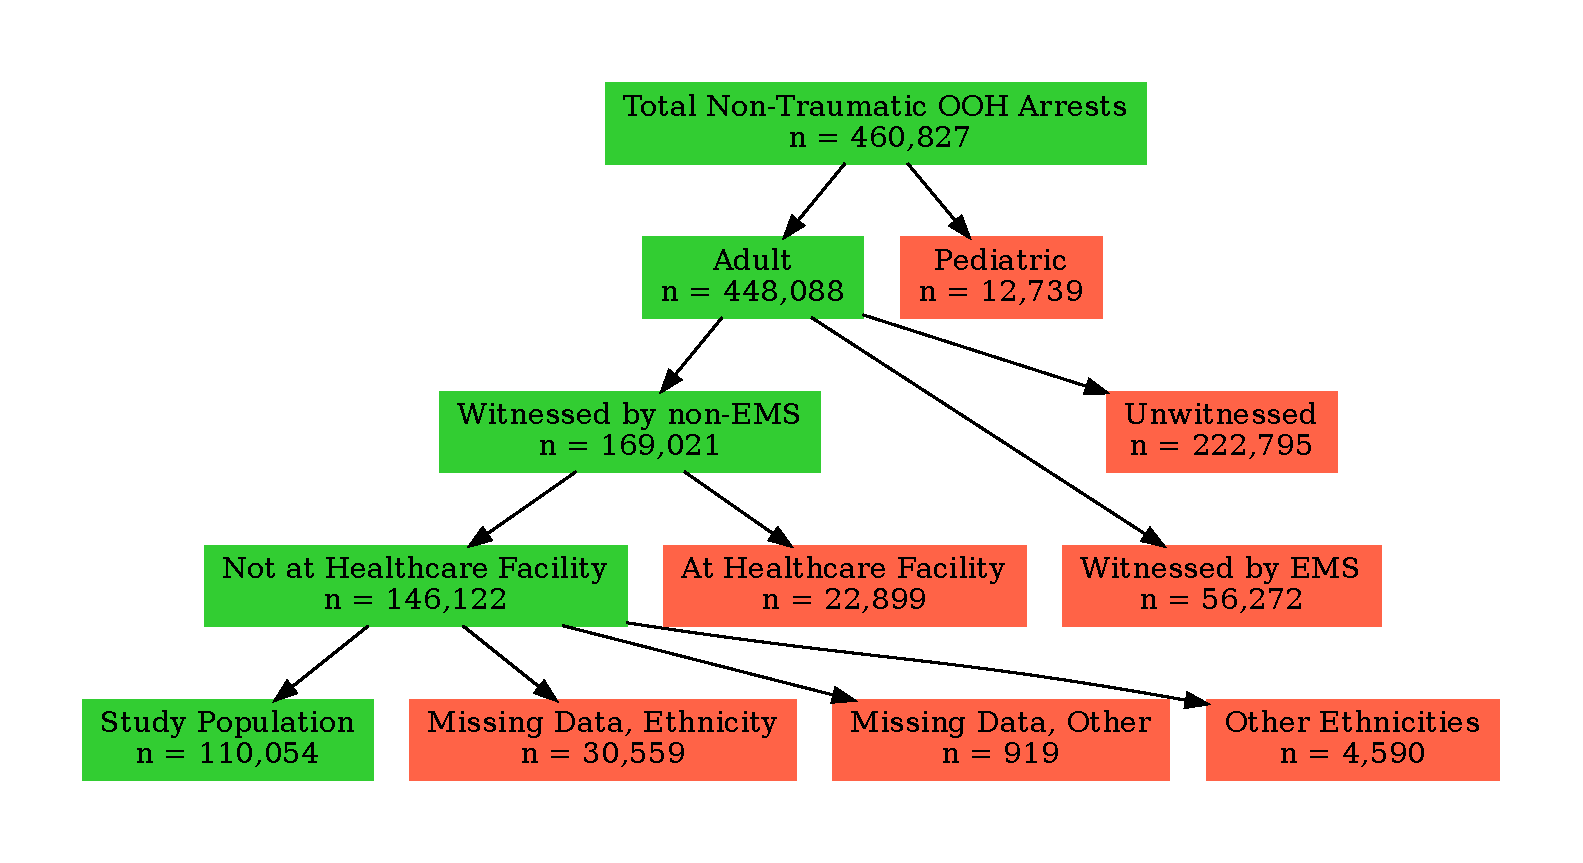
\includegraphics[width=1\linewidth]{fig_cpr-outcomes}
					\label{fig:figcpr-outcomes}
				\end{figure}
			\end{frame}
	\subsection{Methods}
		\begin{frame}
			\textbf{Statistical Methods}
					\begin{itemize}
						\tiny
						\item ``We analyzed the incidence of bystander CPR according to the race or ethnic group of persons who had out-of-hospital cardiac arrests that occurred at home and in public locations. Analyses were further \textbf{stratified} according to the racial or ethnic makeup and the income composition of the neighborhood in which the arrest occurred.''
						\item ``To assess for racial and ethnic differences in the incidence of bystander CPR, multivariable \textbf{hierarchical logistic regression models} were constructed separately for out-of-hospital cardiac arrests that occurred at home and those that occurred in public locations. ''
						\item ``Besides race and ethnic group, these models adjusted for the age and sex of the person who had a cardiac arrest, the calendar year of arrest, the cause of the arrest (presumed cardiac, respiratory, or other), and urbanicity (according to U.S. census urban–rural tract classification: urbanized [$\geq 50,000$ residents], urban cluster [non-urbanized areas,$\geq 2500$ residents]; or rural [$\leq$ 2500 residents]) as \textbf{fixed effects}.''
						\item ``In all models, the effect of race was categorized according to \textbf{between-cluster and within-cluster effects}, with the latter representing the association between the race or ethnic group of a person who had an arrest and the likelihood of bystander CPR within an individual neighborhood.''
					\end{itemize}
				\end{frame}
				\begin{frame}
					\textbf{Statistical Methods}
					\begin{itemize}
						\tiny
						\item``To examine whether racial and ethnic differences in bystander CPR were explained by neighborhood factors, we repeated the above analyses of out-of-hospital cardiac arrests that occurred at home and in public locations for each neighborhood racial or ethnic-group designation and each
						income strata.''
						\item ``The analyses for survival to hospital discharge and favorable neurologic survival initially were adjusted for the same variables that were used for the outcome of bystander CPR. \textbf{The analyses were further adjusted for the presence or absence of bystander CPR and the cardiac-arrest rhythm that was initially detected. }''
						\item ``We constructed a hierarchical model for arrests in a public location and adjusted for the age and sex of the person who had the arrest, calendar year, the race or ethnic group of the person, the cause of the arrest (i.e., cardiac, respiratory, other), urbanicity, public location category, neighborhood racial and ethnic makeup, and neighborhood income.''
					\end{itemize}
		\end{frame}
		\begin{frame}
				\frametitle{Methods: Explanations}
					\begin{itemize}
						\item Stratified analyses
						\item Hierarchical logistic regression model
						\item Fixed effects
						\item Between- versus within-cluster effects
					\end{itemize}
		\end{frame}
		\begin{frame}
			\frametitle{Stratified Analyses}
				\begin{itemize}
					\item Picking a sample from a population
					\item How do we pick a \textit{representative} sample?
						\begin{itemize}
							\item Simple random sample
							\item Stratified sample
						\end{itemize}
				\end{itemize}
		\end{frame}
		\begin{frame}
			\centering
			\begin{figure}
				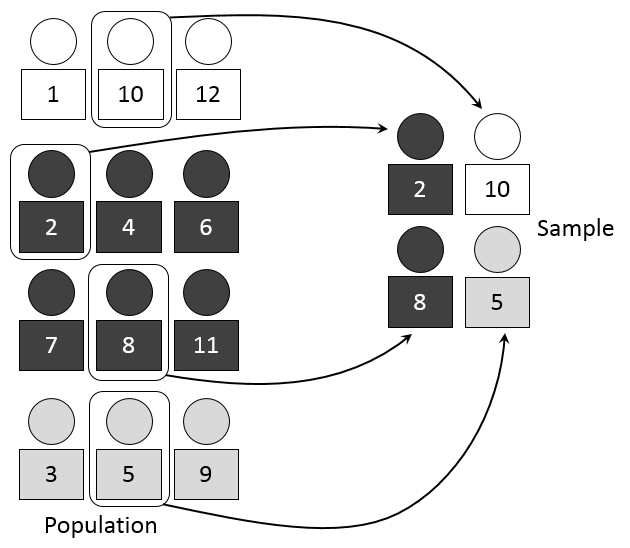
\includegraphics[width=0.7\linewidth]{img/stratified-sampling}
				\label{fig:stratifiedsampling}
			\end{figure}
		\tiny Source: \href{https://commons.wikimedia.org/wiki/File:Stratified\_sampling.PNG}{Dan Kernler, https://commons.wikimedia.org} 
		\end{frame}
		\begin{frame}
			\frametitle{Hierarchical Logistic Regression Model}
				\begin{itemize}
					\item Three key words:
					\begin{itemize}
						\item Regression
							\begin{itemize}
								\item Fitting a line (or other function) to data
							\end{itemize}
						\item Logistic
						\begin{itemize}
							\item  Logistic regression is used when the dependent variable is binary  in nature.
							\item Logistic function is an S-shaped (sigmoid) curve 
						\end{itemize}
						\item Hierarchical
							\begin{itemize}
								 \item ``Hierarchical'' is sometimes used to refer to random / mixed effects models (because parameters sit in a hierarchy).
							\end{itemize}
					\end{itemize}
				\end{itemize}
		\end{frame}
		\begin{frame}
			Linear Regression
			\begin{figure}
				\centering
				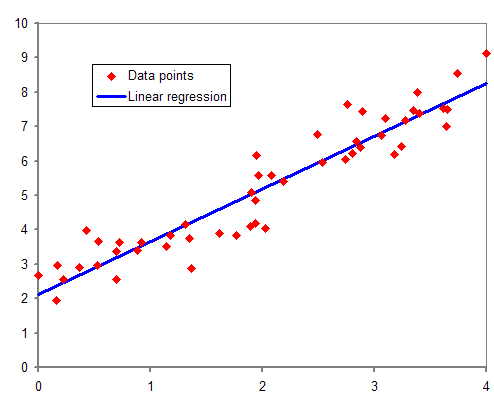
\includegraphics[width=0.7\linewidth]{img/linear-regression}
				\label{fig:linear-regression}
			\end{figure}
		\end{frame}
		\begin{frame}
			Logistic Curve
		\begin{figure}
			\centering
			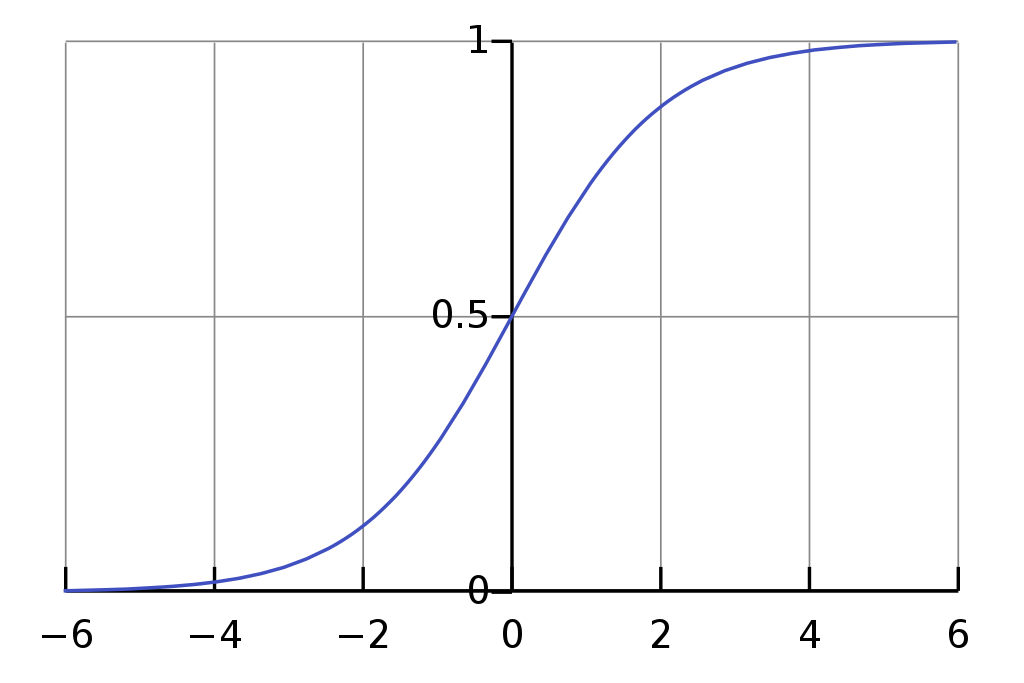
\includegraphics[width=0.8\linewidth]{img/logistic-curve}
			\label{fig:logistic-curve}
		\end{figure}
	\end{frame}
	\begin{frame}
		Logistic Curve, Example
		\begin{figure}
			\centering
			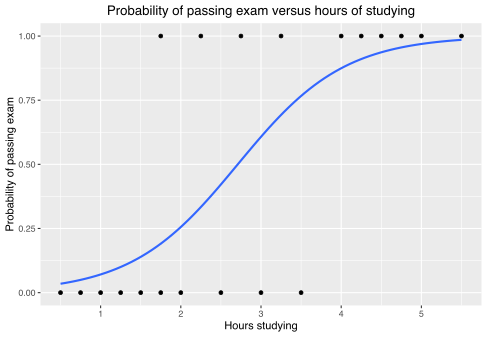
\includegraphics[width=0.8\linewidth]{img/exam-pass-logistic-curve}
			\label{fig:exam-pass-logistic-curve}
		\end{figure}
	\end{frame}
	\begin{frame}
			\frametitle{Fixed Effects}
				\begin{itemize}
					\item Fixed effects model
						\begin{itemize}
							\item  Regression model in which the group means are fixed (non-random) 
						\end{itemize}
					\item Random effects
						\begin{itemize}
							\item A model in which the group means are a random sample from a population
						\end{itemize}
					\item What does this mean?
					\begin{itemize}
						\item Study chose to assume certain elements in their model would have a \textbf{fixed} (as opposed to random) effect size
					\end{itemize}
				\end{itemize}
		\end{frame}
		\begin{frame}
			\textbf{Statistical Methods}
			\begin{itemize}
				\tiny
				\item ``We analyzed the incidence of bystander CPR according to the race or ethnic group of persons who had out-of-hospital cardiac arrests that occurred at home and in public locations. Analyses were further \textbf{stratified} according to the racial or ethnic makeup and the income composition of the neighborhood in which the arrest occurred.''
				\item ``To assess for racial and ethnic differences in the incidence of bystander CPR, multivariable \textbf{hierarchical logistic regression models} were constructed separately for out-of-hospital cardiac arrests that occurred at home and those that occurred in public locations. ''
				\item ``Besides race and ethnic group, these models adjusted for the age and sex of the person who had a cardiac arrest, the calendar year of arrest, the cause of the arrest (presumed cardiac, respiratory, or other), and urbanicity (according to U.S. census urban–rural tract classification: urbanized [$\geq 50,000$ residents], urban cluster [non-urbanized areas,$\geq 2500$ residents]; or rural [$\leq$ 2500 residents]) as \textbf{fixed effects}.''
				\item ``In all models, the effect of race was categorized according to \textbf{between-cluster and within-cluster effects}, with the latter representing the association between the race or ethnic group of a person who had an arrest and the likelihood of bystander CPR within an individual neighborhood.''
			\end{itemize}
		\end{frame}
	
	\subsection{Results}
		\begin{frame}
			\begin{figure}
					\centering
					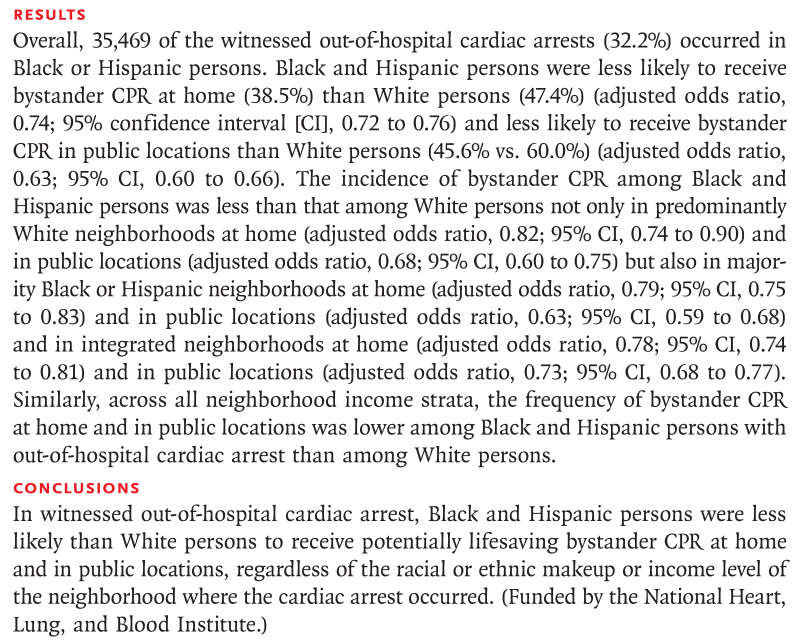
\includegraphics[height=0.9\textheight, keepaspectratio]{img/results}
					\label{fig:results}
				\end{figure}
		\end{frame}
		\begin{frame}
			\frametitle{Results over Time}
			\begin{figure}
				\centering
				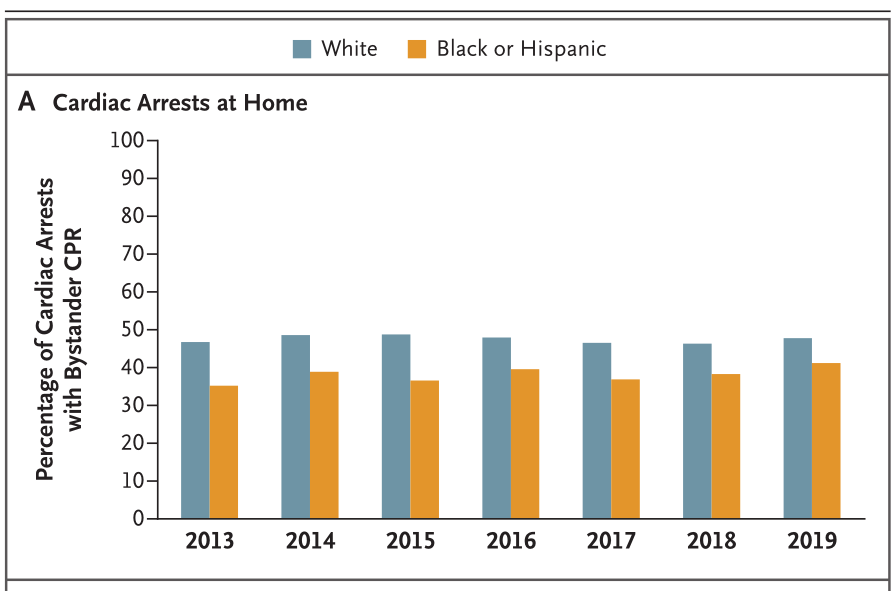
\includegraphics[height=0.6\linewidth]{img/fig1-part1}
				\label{fig:fig1-part1}
			\end{figure}
		\end{frame}
		\begin{frame}
			\frametitle{Results over Time}
			\begin{figure}
				\centering
				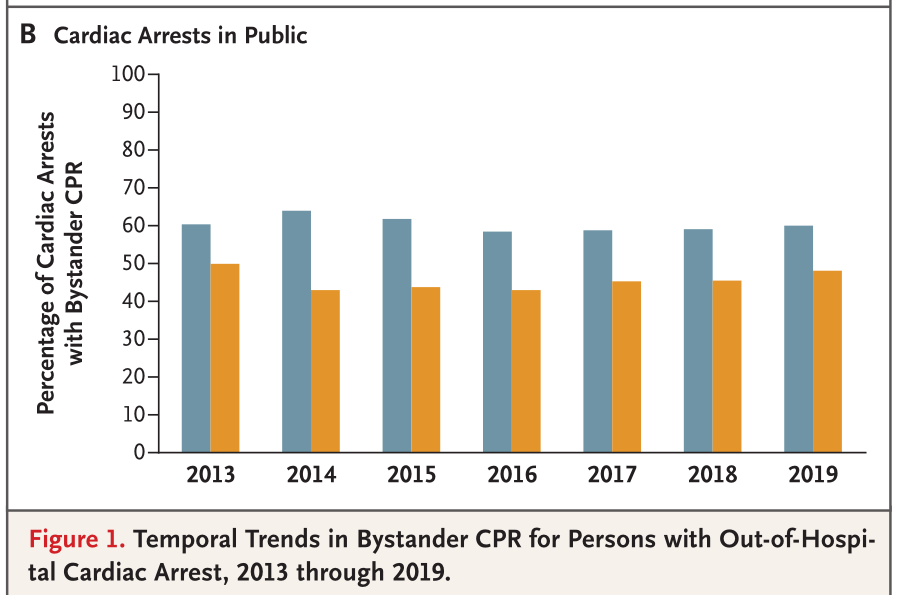
\includegraphics[height=0.6\linewidth]{img/fig1-part2}
				\label{fig:fig1-part2}
			\end{figure}
		\end{frame}
		\begin{frame}
			\frametitle{Results by Variable}
			\pause
			\begin{figure}
				\centering
				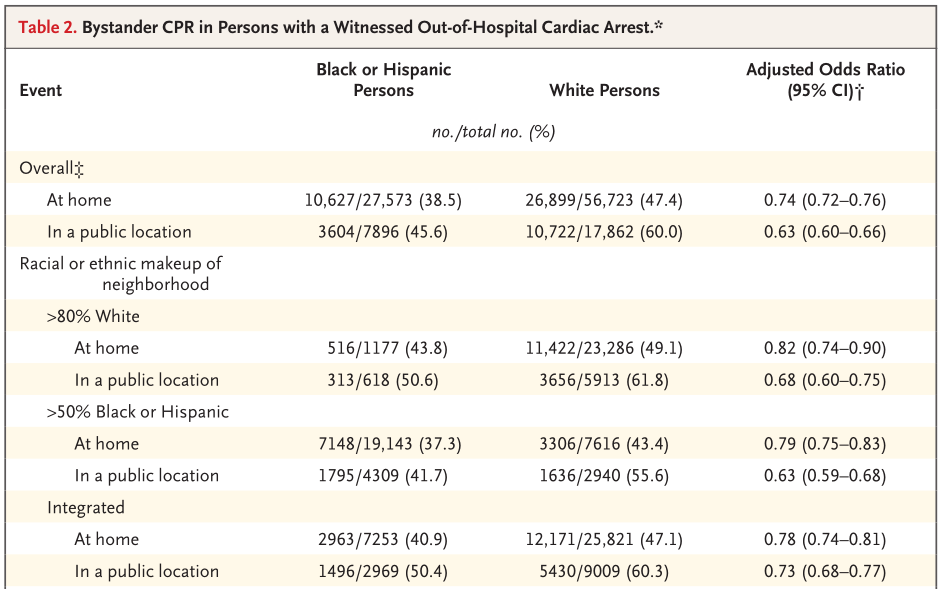
\includegraphics[width=1.0\linewidth]{img/table2-part1.png}
				\label{fig:tab2-part1}
			\end{figure}
		\end{frame}
		\begin{frame}
			\frametitle{Results by Variable}
			\begin{figure}
				\centering
				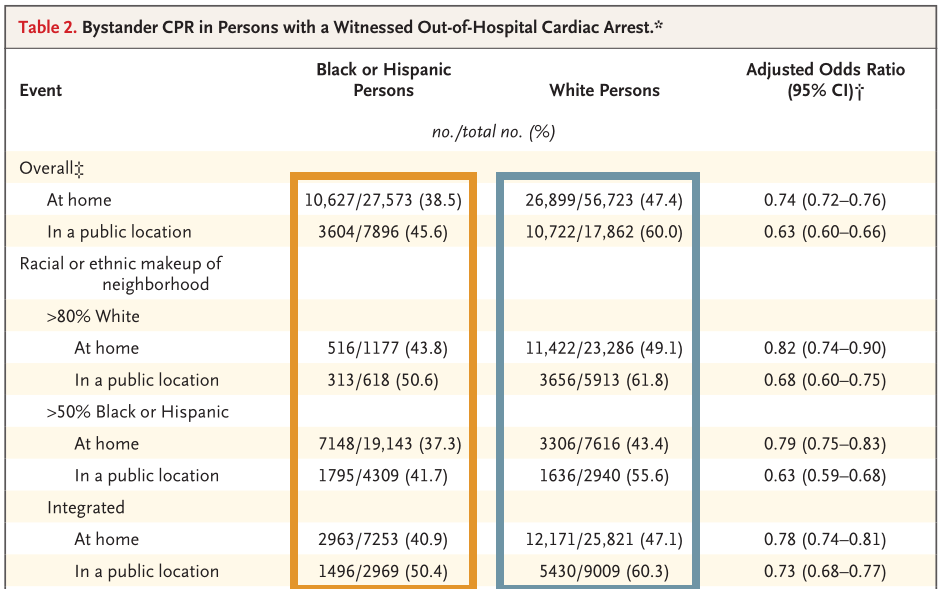
\includegraphics[width=1.0\linewidth]{img/table2-part1-boxed.png}
				\label{fig:tab2-part1-boxed}
			\end{figure}
		\end{frame}
		\begin{frame}
			\frametitle{Results by Variable}
			\begin{figure}
				\centering
				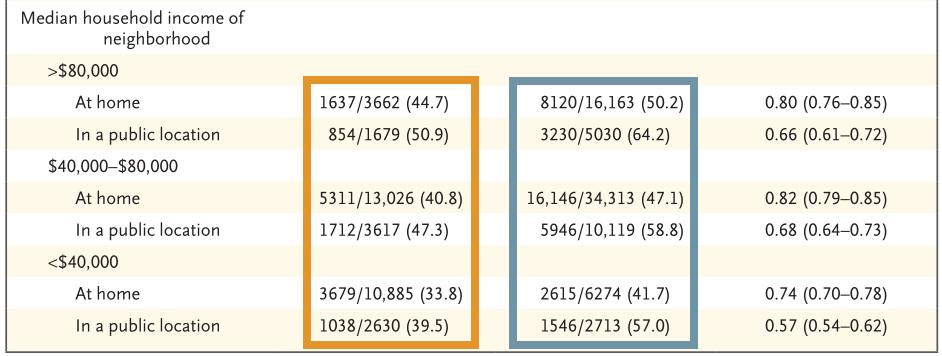
\includegraphics[width=1.0\linewidth]{img/table2-part2-boxed.png}
				\label{fig:tab2-part2-boxed}
			\end{figure}
		\end{frame}
		\begin{frame}
			\frametitle{Changes with Public Location?}
			\pause
			\begin{figure}
				\centering
				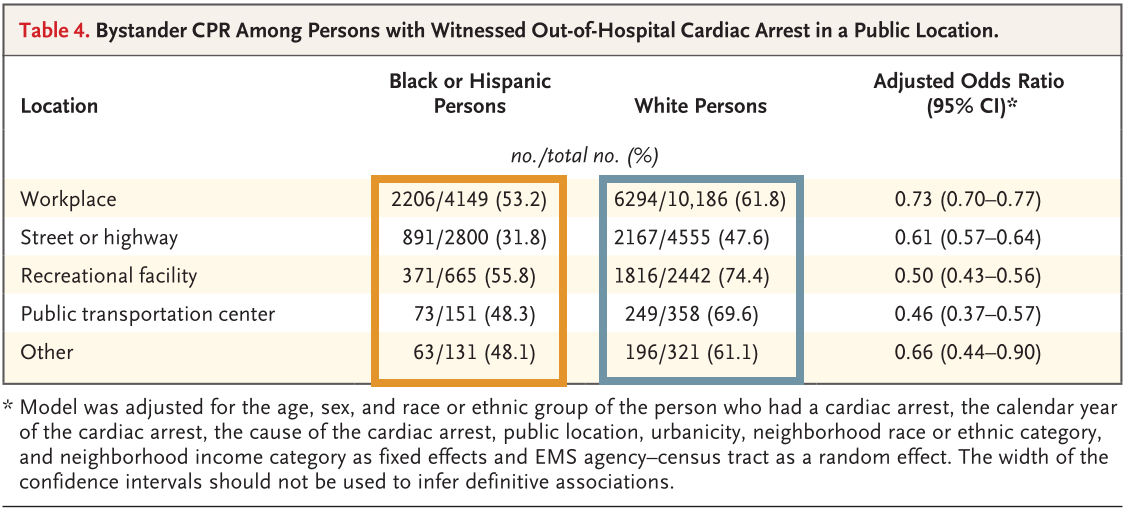
\includegraphics[width=1.0\linewidth]{img/table4-boxed}
				\label{fig:tab4-boxed}
			\end{figure}
		\end{frame}
		\begin{frame}
			\frametitle{Outcomes in OOH Cardiac Arrest}
			\pause
			\begin{figure}
				\centering
				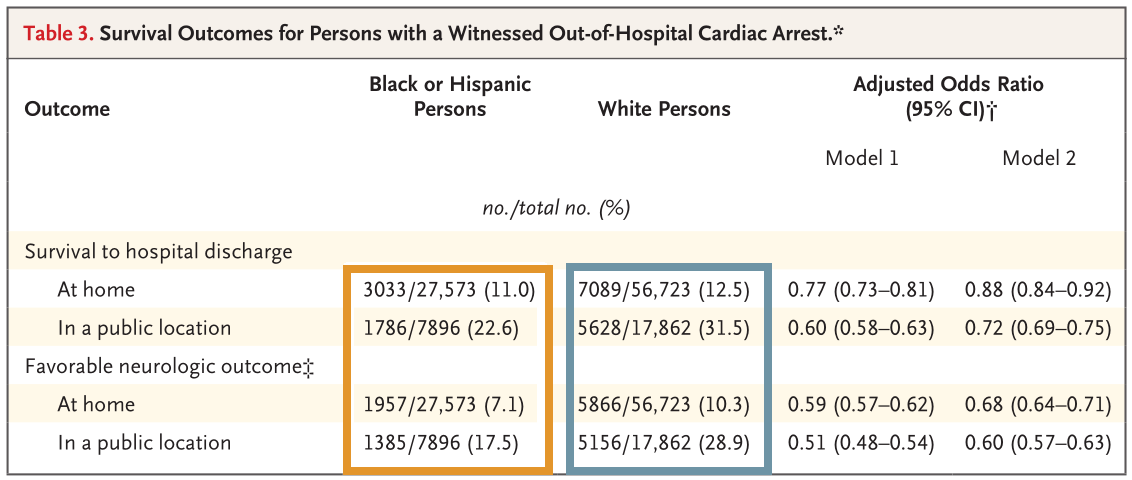
\includegraphics[width=1.0\linewidth]{img/table3-boxed}
				\label{fig:tab3-boxed}
			\end{figure}
		\pause
		``Differences according to race and ethnic group in survival outcomes were attenuated with further adjustment for receipt of bystander CPR and initial cardiac arrest rhythm [see Model 2].''
		\end{frame}
	\subsection{Discussion}
		\begin{frame}
			\frametitle{Why These Results?}
				\begin{itemize}
					\item Prior explanations didn't hold
						\begin{itemize}
							\item If product of lower CPR training rates, why persistent differences in white and/or wealthy neighborhoods?
						\end{itemize}
					\item New hypotheses
						\begin{itemize}
							\item Structural racism
							\item Implicit or explicit biases
						\end{itemize}
					\item Limitation
						\begin{itemize}
							\item Bystander race unknown
						\end{itemize}
				\end{itemize}
		\end{frame}
\section{Assessing the Study}
	\subsection{Dealing with Imperfect Data}
		\begin{frame}
			\frametitle{Dealing with Imperfect Data}
				\begin{itemize}
					\item How do we know our data is good?
					\item What do we do about missing data?
					\item What difference is (clinically) meaningful?
					\item Does testing itself affect our conclusions?
				\end{itemize}
		\end{frame}
		\subsubsection*{Classification Errors}
			\begin{frame}
				\frametitle{Classification Errors}
				- p. 1571 :: ``...race and ethnic group are reported by persons who had a cardiac arrest or their family members, whenever possible, or are reported by EMS personnel when the person dies during resuscitation and no family member or acquaintance is available to provide race or ethnic-group information.''
				\begin{itemize}
					\item Problems with this?
				\end{itemize}
			\end{frame}
		\subsubsection*{Missing Data}
			\begin{frame}
				\frametitle{Missing Data}
				- p. 1572 :: ``To account for potential bias owing to missing data regarding race or ethnic group, we used inverse probability weighting to generate all model estimates.''
				\begin{itemize}
					\item What does this mean?
					\item Why does missing data matter?
				\end{itemize}
			\end{frame}
						\begin{frame}
				\frametitle{Significant Missing Data}
				\begin{figure}
					\centering
					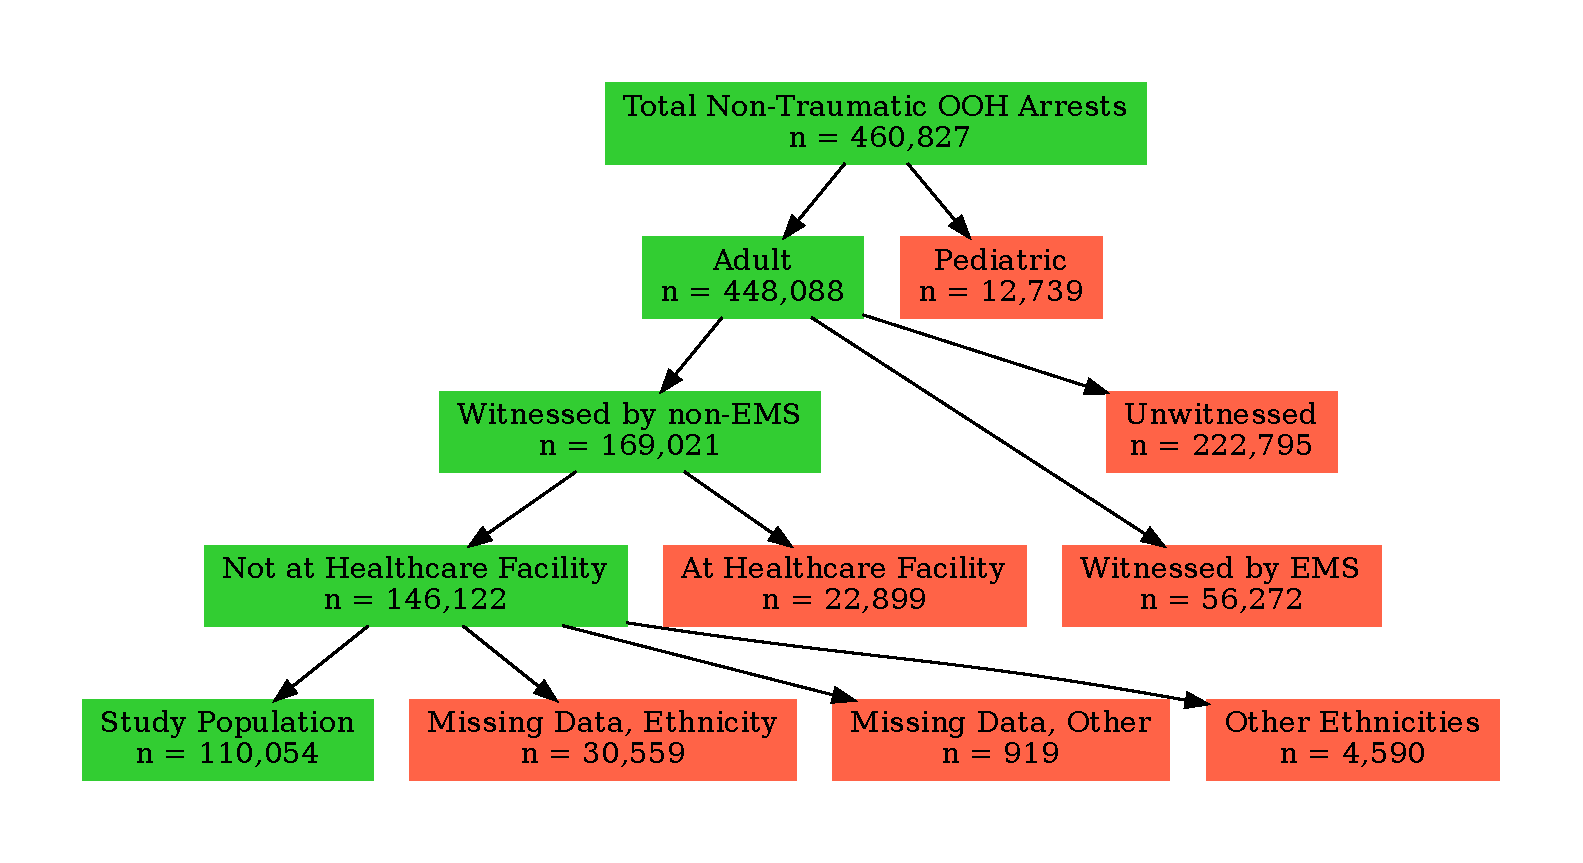
\includegraphics[width=1\linewidth]{fig_cpr-outcomes}
					\label{fig:figcpr-outcomes-}
				\end{figure}
			\end{frame}
			\begin{frame}
				\frametitle{Missing Data, Techniques}
				\begin{itemize}
					\item How can data go missing?
						\begin{itemize}
							\item Missing completely at random
							\item Missing at random
							\item Missing not at random
							\item Example: depression screening in men
						\end{itemize}
					\pause
					\item How can we deal with missing data?
						\begin{itemize}
							\item Imputation
								\begin{itemize}
									\item ``filling in'' missing values (mean substitution, regression, multiple imputations)
								\end{itemize}
							\item Omission
								\begin{itemize}
									\item withold data with missing values from analysis
								\end{itemize}
							\item Analysis
								\begin{itemize}
									\item use methods unaffected by the missing values
								\end{itemize}
						\end{itemize}
				\end{itemize}	
			\end{frame}
			\begin{frame}
				\frametitle{Missing Data}
				- p. 1572 :: ``To account for potential bias owing to missing data regarding race or ethnic group, we used \textbf{inverse probability weighting }to \textit{generate} all model estimates.''
				\pause
				\begin{itemize}
					\item authors used \textit{imputation}
					\item logisitc regression model (think fitting to a line)
				\end{itemize}
			\end{frame}
	\subsection{Mapping Results to Conclusions}
		\subsubsection*{MCID}
			\begin{frame}
				\frametitle{MCID: Minimal Clinically Important Difference}
				``Owing to the large sample size, characteristics of Black or Hispanic persons and White persons at baseline were compared with the use of standardized differences, in which a standardized absolute difference of more than 10 percentage points was considered clinically meaningful.''
			\end{frame}
			\begin{frame}
				\frametitle{MCID: Minimal Clinically Important Difference}
				\begin{figure}
					\centering
					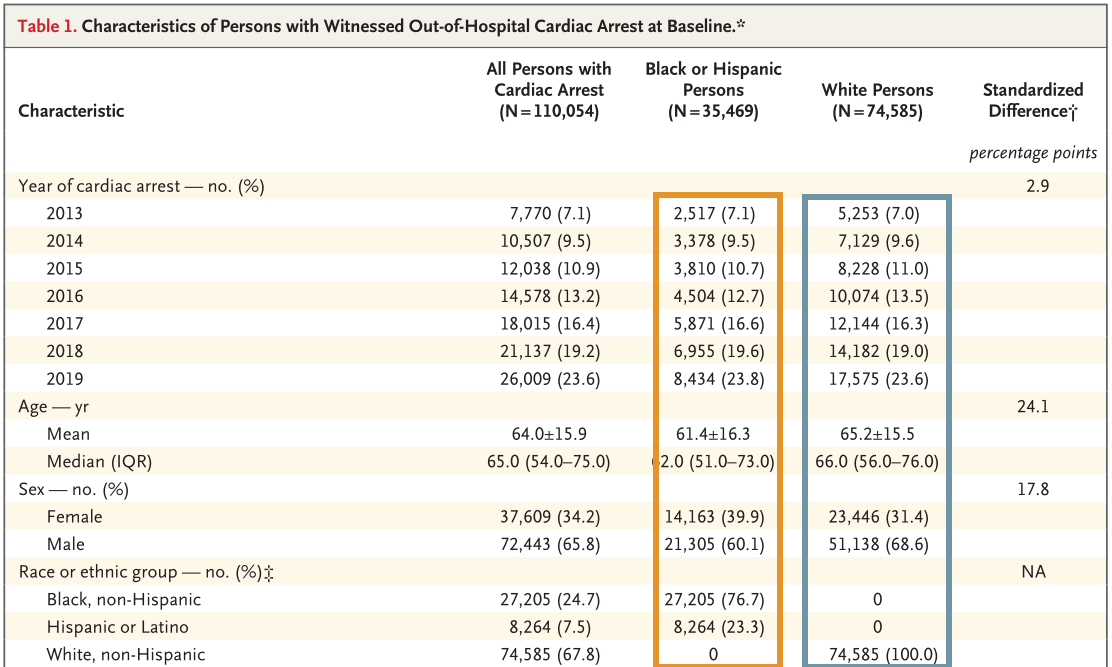
\includegraphics[width=1.0\linewidth]{img/table1-part1-boxed}
					\label{fig:table1-part1-boxed}
				\end{figure}
			\end{frame}
		\begin{frame}
			\frametitle{MCID: Minimal Clinically Important Difference}
			\begin{figure}
				\centering
				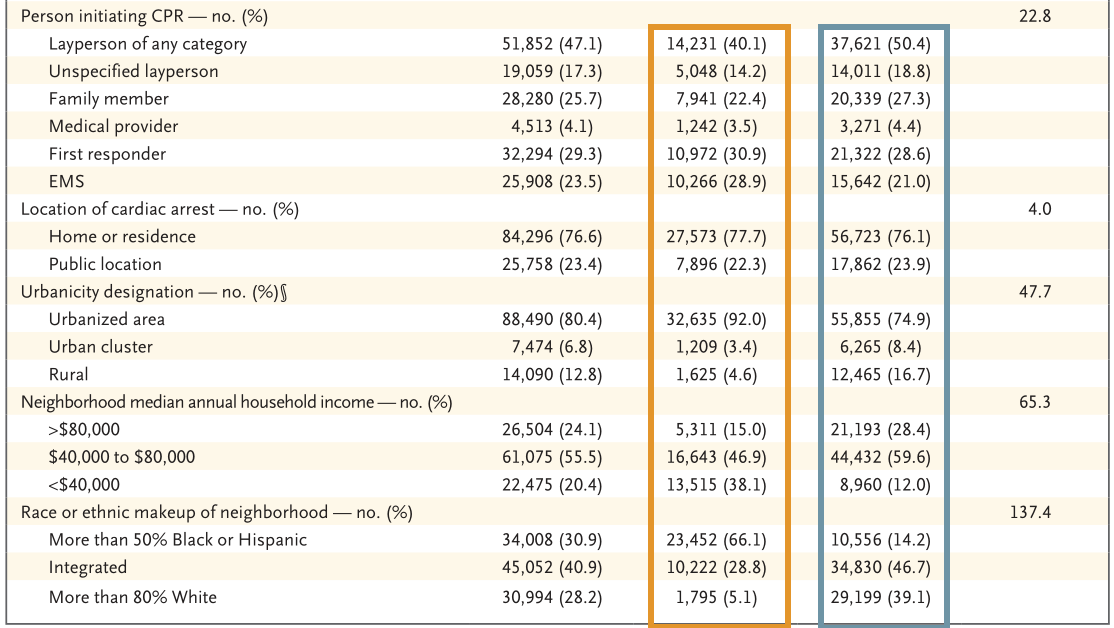
\includegraphics[width=1.0\linewidth]{img/table1-part2-boxed}
				\label{fig:table1-part2-boxed}
			\end{figure}
		\end{frame}
		\subsubsection*{Multiple Comparisons Problem}
			\begin{frame}
				\frametitle{Multiple Comparisons Problem}
					\begin{itemize}
						\item How do we decide if a result is valid / significant?
							\begin{itemize}
								\item p values! (rejecting the ``null hypothesis'')
								\item example when $\alpha = 0.05$
								\pause
							\end{itemize}
						\end{itemize}
							\begin{itemize}
								\item Family-wise error rate (FWER)
									\begin{itemize}
										\item probability of making one or more false discoveries (type I error) when performing multiple hypotheses test
										\item $\alpha_{total} = 1 - (1 - \alpha_{per.comparison})^m$
										\pause
									\end{itemize}
							\end{itemize}
				\begin{center}
					\begin{tabular}{| c | c | c |}
						\hline
						\textbf{Number of tests } & \textbf{$\alpha_{per.comparison}$} & \textbf{FWER} \\
						\hline
						1 & 0.05 & 0.05 \\
						\hline
						5 & 0.05 &  0.23 \\
						\hline
						15 & 0.05 &  0.54 \\
						\hline
						27 & 0.05 &  0.75 \\
						\hline
						100 & 0.05 & 0.994\\
						\hline
					\end{tabular}
				\end{center}
			\end{frame}
			\begin{frame}
				\frametitle{Adjusting for Multiple Testing}
					\begin{itemize}
					\item Bonferroni correction
						\begin{itemize}
							\item $\alpha_{per.comparison}=\frac{\alpha_{total}}{m}$
							\item \textit{e.g.} if $m = 5$ and you want $\alpha_{total} = 0.05$, $\alpha_{per.comparison}=\frac{0.05}{5}=0.01$
						\end{itemize}
					\item Sidak correction
						\begin{itemize}
							\item $\alpha_{sidak} = 1 - (1-\alpha)^{\frac{1}{m}}$
							\item \textit{e.g.} if $m = 10$ and $\alpha_{total} = 0.05$, $\alpha_{per.comparison}= 1 - (1-0.05)^{\frac{1}{10}}= 0.005116$
						\end{itemize}
					\pause
				\item Many others (Tukey's, Holm's, Hocberg's, Dunnett's, harmonic mean procedure, etc.)
					\end{itemize}	
			\end{frame}
		\begin{frame}
			\frametitle{How the Paper Dealt with Multiple Testing}
				p. 1572: ``Because \textbf{we did not prespecify that there would be correction for multiplicity} when conducting tests, results are reported as point estimates and 95\% confidence intervals. The widths of the confidence intervals have not been adjusted for multiplicity, so the intervals should not be used to infer definitive associations.''
		\end{frame}
\section{Takeaway Points}
	\subsection{Study}
		\begin{frame}
			\frametitle{Takeaway Points}
				\begin{itemize}
					\item \textbf{Study}
						\begin{itemize}
							\item Black and Hispanic people get less OOH CPR than Whites
								\begin{itemize}
									\item no amelioration by location, neighborhood income, or neighborhood ethnic makeup
								\end{itemize}
							\pause
							\item Black and Hispanic people have worse outcomes (survival, 	neurologic) from OOH arrests than Whites
							\item Reasons unclear, but may include sequelae of structural racism, implicit or explicit biases, etc.
						\end{itemize}
				\end{itemize}
		\end{frame}
	\subsection{Statistics}
\begin{frame}
	\frametitle{Takeaway Points}
	\begin{itemize}
		\item \textbf{Statistics}
		\begin{itemize}
			\item Paper methods
				\begin{itemize}
					\item stratified analysis, logistic regression model
				\end{itemize}
			\item Missing data matters!
				\begin{itemize}
					\item imputed here, but other studies may not mention
				\end{itemize}
			\item Think about minimal clinically important difference (MCID)
				\begin{itemize}
					\item Statistical significance $\neq$ clinical significance
				\end{itemize}
			\item Remember issues with multiple testing!
				\begin{itemize}
					\item p values and confidence intervals both count!
					\item Did they account for correction?
					\item How should you interpreter p values and confidence intervals?
				\end{itemize}
		\end{itemize}
	\end{itemize}
\end{frame}
\section{References}
	\begin{frame}
		\frametitle{References}
		\printbibliography
	\end{frame}
\end{document}
